\documentclass[ngerman]{dtk}% load class options 07
%%
%% Packete/Style-Optionen und anderes Material in der Pr"aambel:
%%
\usepackage[]{showexpl,ifthen}
\usepackage{xspace,listings,xcolor}
\usepackage[]{babel}
\usepackage[utf8]{inputenc}

\definecolor{hellgelb}{rgb}{1,1,0.8}
\definecolor{colKeys}{rgb}{0,0,1}
\definecolor{colIdentifier}{rgb}{0,0,0}
\definecolor{colComments}{rgb}{1,0,0}
\definecolor{colString}{rgb}{0,0.5,0}

\lstset{%
    float=hbp,%
    basicstyle=\ttfamily\small, %
    identifierstyle=\color{colIdentifier}, %
    keywordstyle=\color{colKeys}, %
    stringstyle=\color{colString}, %
    commentstyle=\color{colComments}, %
    columns=flexible, %
    tabsize=2, %
%    frame=single, %
    extendedchars=true, %
    showspaces=false, %
    showstringspaces=false, %
    backgroundcolor=\color{hellgelb}, %
    breakautoindent=true, %
    captionpos=b%
}

\usepackage{booktabs}

\addbibresource{uweziegenhagen.bib}

\begin{document}


\title{Dynamisches Ausblenden von Text und Erstellung von Lückentexten}

\Author{Uwe}{Ziegenhagen}{Köln}

\maketitle

\markboth{Dynamisches Ausblenden}{Dynamisches Ausblenden}

%%-----------------------------------------------------------------------------
\begin{abstract}
Anwendungen für das dynamische Ausblenden von Textteilen gibt es viele: Ein Lebenslauf soll mal mit, mal ohne Angabe von Abschlussnoten gesetzt werden, für die Schule sollen Aufgabenblätter mal mit, mal ohne Lösungsweg erstellt werden. 

Ebenfalls beliebt in der Schule ist das Erstellen von Lückentexten, in denen statt des Lösungswortes nur eine entsprechende Anzahl von Unterstrichen oder ähnlichen Zeichen findet. Mit \LaTeX{} ist es recht einfach, solche Anforderungen umzusetzen, bei der Gelegenheit lässt sich auch den Umgang mit Befehlsdefinitionen üben.
\end{abstract}

\section{Ausblenden über die Textfarbe}

Über das Setzen der Textfarbe auf weiss lässt sich Text zwar optisch ausblenden -- was für reine Druckdokumente zwar ausreichend sein mag, in der PDF-Datei lässt sich der ausgeblendete Text aber markieren und in die Zwischenablage kopieren

\begin{LTXexample}[pos=t]
\documentclass{article}
\usepackage{xcolor}
\newcommand{\blende}[1]{%
\textcolor{white}{#1}}

\begin{document}

Hallo, ich bin ein Text, in dem das Wort 
\blende{Phantom} ausgeblendet wird. 

\end{document}
\end{LTXexample}


\section{Text verstecken mit \textbackslash \texttt{phantom\{\}}}

Um auch in elektronischen Dokumenten Textteile wirksam auszublenden, stellt \TeX\xspace den \verb|\phantom| Befehl bereit. Im folgenden Beispiel wird der \verb|\blende| Befehl in einem ersten Ansatz doppelt definiert. Je nachdem, ob ausgeblendet werden soll oder nicht, wird entweder die eine oder die andere Definition genutzt.

\begin{LTXexample}[pos=t]
\documentclass{article}
\newcommand{\blende}[1]{\phantom{#1}}
%\newcommand{\blende}[1]{#1}

\begin{document}

Hallo, ich bin ein Text, in dem das Wort \blende{Phantom} 
ausgeblendet wird. 

\end{document}
\end{LTXexample}

Das manuelle Auskommentieren von Befehlen ist nicht sonderlich elegant, daher können wir mithilfe des \texttt{ifthen}-Pakets \cite{ifthen} ein entsprechendes Schalterkommando definieren, das über die Werte \texttt{true} oder \texttt{false} die Definition des richtigen \verb|\blende| Kommandos übernimmt.

Die Syntax des Befehls lautet \verb|\ifthenelse{Bedingung}| \verb|{true-Teil}| \verb|{false-Teil}|, \verb|Bedingung| ist dabei ein boolescher Ausdruck. Im \verb|{true-Teil}| stehen die Befehle, die ausgeführt werden, wenn dieser Ausdruck 'wahr' ergibt, im  \verb|{false-Teil}| die Befehle, die bei 'falsch' ausgeführt werden.

Wenn die Variable \texttt{ausblenden} auf 'true' gesetzt ist, wird \verb|\blende| mit \verb|\phantom| Aufruf definiert, ansonsten erfolgt nur die einfache Ausgabe des als Parameter übergebenen Texts.

Über eine Änderung der Befehlsdefinition können wir das Beispiel noch deutlich einfacher gestalten. Das Kommando \verb|\blende{}| wird nur einmal definiert, in der Definition wird überprüft, ob der boolesche Ausdruck \verb|ausblenden| auf 'true' oder 'false' gesetzt ist und der übergebene Text entweder mit oder ohne \verb|\phantom| Aufruf ausgegeben.

\begin{LTXexample}[pos=t]
\documentclass{article}
\usepackage{ifthen}
\newboolean{ausblenden}
\setboolean{ausblenden}{true} 

\ifthenelse{\boolean{ausblenden}}
		{\newcommand{\blende}[1]{\phantom{#1}}} % der TRUE-Teil
		{\newcommand{\blende}[1]{#1}} % der FALSE-Teil 

\begin{document}

Hallo, ich bin ein Text, in dem das Wort \blende{Phantom} 
ausgeblendet wird.

\end{document}
\end{LTXexample}


\begin{LTXexample}[pos=t]
\documentclass{article}
\usepackage{ifthen}
\newboolean{ausblenden}
\setboolean{ausblenden}{true} 

\newcommand{\blende}[1]{%
\ifthenelse{%
\boolean{ausblenden}}
{\phantom{#1}}%
{#1}}

\begin{document}

Hallo, ich bin ein Text, in dem das 
Wort \blende{Phantom} ausgeblendet wird. 

\end{document}
\end{LTXexample}


\section{Das \texttt{ifthen}-Paket}

Abgesehen von der oben vorgestellten Nutzung des \texttt{ifthen} Pakets zur Steuerung von Befehlsdefinitionen kann es natürlich auch allein genutzt werden, um Textteile auszublenden. Das folgenden Beispiel zeigt noch einmal die minimalen Einstellungen, um Text per \texttt{ifthen} auszublenden.

\begin{LTXexample}[pos=t]
\documentclass[]{article}
\usepackage{ifthen}

\newboolean{greeting}
\setboolean{greeting}{true} 

\begin{document}

\ifthenelse{\boolean{greeting}}{Hier steht der Text, der bei 
greeting=true gesetzt wird.}{Hier steht der Text, der bei 
greeting=false gesetzt wird}

\end{document}
\end{LTXexample}

\section{Erstellung von Lückentexten}

Bei der Erstellung von Lückentexten wird normalerweise nicht nur der Text ausgeblendet, es wird auch eine visuelle Unterstützung in Form einer Linie oder einer Folge von Unterstrichen gegeben, die einen Hinweis auf die Länge des einzutragenden Wortes gibt.

Für die Erstellung von Lückentexten können wir die Befehlsdefinition etwas abändern. Basierend auf einem Codeschnipsel aus dem Internet \cite{almer} können wir unser Beispiel abändern:

Für jedes Wort, das ausgeblendet werden soll, setzt dieser \verb|\luecke{}| Befehl eine gepunktete Lücke von der 2,7-fachen Länge des übergebenen Textes. Der Verlängerungsfaktor von 2,7 ist hier nur ein Richtwert, der in auch in Abhängigkeit von Schriftart, Zeilenabstand und ähnlichen Einflussfaktoren adjustiert werden sollte. 

\begin{LTXexample}[pos=t]
\documentclass{article}
\usepackage{ifthen}
\newboolean{lueckentext}
\setboolean{lueckentext}{true} 

\newcommand{\luecke}[1]{%
\ifthenelse{\boolean{lueckentext}}{
	\newlength{\lueckenbox}
	\settowidth{\lueckenbox}{#1}
\raisebox{-1.0ex}%
{\parbox{2.7\lueckenbox}%
{\dotfill}}}%
{#1}}

\begin{document}

\noindent Hallo, ich bin ein Text, in dem das Wort 
\luecke{Phantom} ausgeblendet wird. 

\end{document}
\end{LTXexample}

Möchte man die Anzahl der Buchstaben kenntlich machen, die der ausgeblendete Text hat, kann man die folgende Definition nutzen. Sie nutzt den \verb|\StrLen| Befehl aus dem \texttt{xstring} Paket, um die Länge des übergebenen Textes in \verb|\laenge| zu speichern. über die FOR-Schleife aus dem \texttt{forloop} Paket wird dann für jedes Zeichen wird ein \textunderscore\xspace gesetzt. Das abschließende \verb|\xspace| dient dann dem korrekten Setzen bzw. Nicht-Setzen von Leerzeichen innerhalb bzw. am Ende eines Satzes.


\begin{lstlisting}[language={[LaTeX]TeX}]
\documentclass{article}
\usepackage{xstring}
\usepackage{forloop}
\usepackage{ifthen,xspace}
\newcounter{cta}% 

\newcommand{\lueckentext}[1]{%
\StrLen{#1}[\laenge]%
\forloop{cta}{0}%
{\value{cta}<\laenge}% 
{\textunderscore\quad}\xspace}%

\begin{document}

\noindent Hallo, ich bin ein Text, in dem das Wort 
\lueckentext{Phantom} ausgeblendet wird. Der Text 
kann auch am Ende stehen \lueckentext{Phantom}! Er
kann aber \lueckentext{auch mehrere Worte} umfassen.
\end{document}
\end{lstlisting}

\begin{figure}[h]
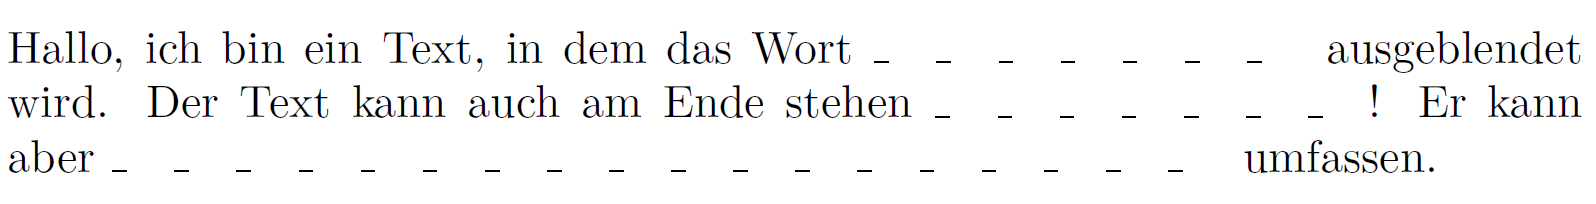
\includegraphics[width=\textwidth]{luecke.png}
\end{figure}

%
%\section{Das \texttt{version}-Paket}
%\url{http://www.tex.ac.uk/tex-archive/macros/latex/contrib/misc/version.sty}

\section{Zusammenfassung}

Durch kleine selbstgeschriebene Codeschnipsel oder das vorgestellte \verb|ifthen| Paket ist es sehr leicht, mit \LaTeX\xspace Dokumente zu erstellen, die in Abhängigkeit eines Parameter Textteile ausblenden oder mit einer Lücke versehen.

Die Befehlsdefinition des Lückentextes ist hinreichend einfach, um an diesem Beispiel in einer der nächsten Ausgaben der DTK die Erstellung eines kleinen \LaTeX-Pakets zu zeigen.  

Anmerkungen und Anregungen zu diesem Artikel sind jederzeit willkommen, die Beispiel habe ich auch auf \url{http://www.uweziegenhagen.de} ablegt.


\end{document}